
\chapter{مفاهیم مربوط به شبکه‌‌های اجتماعی و اجزای فرایند پخش اطلاعات}
%\minitoc
\newpage

\section{مقدمه}
\noindent {
در این فصل در ابتدا به معرفی شبکه‌های اجتماعی آنلاین و مفاهیم مرتبط پیرامون آن‌ها مانند هوموفیلی و فرضیه قدرت اتصال‌ها و همین‌طور شرح نمود گرافی این شبکه‌ها می پردازیم. در ادامه تعریفی از فرایند پخش اطلاعات به موضوع یکی از فرایند‌های مهم در جریان شبکه‌های اجتماعی آنلاین ارایه می دهیم. به همراه مابقی تعاریف مرتبط مانند میم و اقتصاد توجه، در انتها به جمع‌بندی آنچه گفته شد می‌پردازیم. 

}

%\newpage
\section{شبکه‌‌های اجتماعی آنلاین}
\begin{persian}
\noindent
یک شبکه‌ی اجتماعی متشکل از مجموعه‌ای از افراد می‌باشد که با‌هم به گونه‌ای رابطه دارند \cite{easley_networks_2010}. وجود شبکه‌های اجتماعی پدیده‌ای نوع و تازه نمی‌باشد، ولی ظهور اینترنت و در پی آن برپا‌شدن سایت‌‌‌هایی مثل توییتر و فیسبوک که چندصد میلیون کاربر فعال در لحظه را به‌هم متصل می‌کنند سبب از بین رفتن خیلی از محدودیت‌های مکانی و جغرافیایی‌ گذشته برای تشکیل اجتماعات مجازی آنلاین شده است. مثلا فیسبوک در طول‌یک ماه به طور متوسط در حدود ۱ میلیارد\زیرنویس{ فیسبوک به کاربری که در ۳۰ روز گذشته به حساب خود وارد شده باشد و با دیگر اعضا به تعامل پرداخته باشد کاربر فعال می‌گوید.} \cite{taxidou_realtime_2013} کاربر فعال دارد، کاربران توییتر هم که از مرز چند صد میلیون گذشته اند روزانه حدود ۴۰۰ میلیون توییت ارسال می‌کنند. به طور دقیق‌تر این دو سایت و دیگر وبسایت‌های اجتماعی آنلاین سرویس‌هایی شامل دراختیار قراردادن صفحه‌ای اختصاصی برای پیام‌‌ها و محتوای تولیدشده توسط کاربر ارایه می دهند. این امر امکان ارتباط کاربر با کاربران دیگر و پیگیری و به‌اشتراک‌قراردادن محتوا با دیگران را فراهم می سازد 
\cite{guille_information_2013}.
\\\indent
از لحاظ بزرگی ابعاد داده‌ی تولیدی کاربران این سایت‌ها، چگونگی استخراج دانش و اطلاعات‌ کاربران یکی از بحث‌های داغ روز در حوزه‌ی ابر داده\پانویس { Big Data} می‌باشد. برای مثال می‌قدرت ادعا کرد که داده‌ی تولیدی از توییت‌های\footnote{ توییت به پیام‌هایی اطلاق می‌شود که کاربران توییتر می‌قدرتند تولید و ارسال کنند. این پیام ‌‌ها از کم تر از ۱۴۱ حرف تشکیل می‌شوند و می‌قدرتند به همراه هشتگ(رشته‌ای از حروف که با \lr{\#} شروع شود.) و‌یا فایل تصویری و‌یا فیلم و پیوند ارسال شوند.} کاربران توییتر پیچیده‌ترین نوع داده‌ی تولید‌شده در سطح وب می‌باشد \cite{krishnan_data_2013}.
به طور کلی‌ یکی از موارد مطرح امروزی پیرامون این سایت‌ها چگونگی استفاده از این دریای اطلاعات برای حل مشکلاتی می‌باشد که تا چندی‌پیش حلشان غیر ممکن می‌نمود.
 \begin{figure}[H]
 \centering
 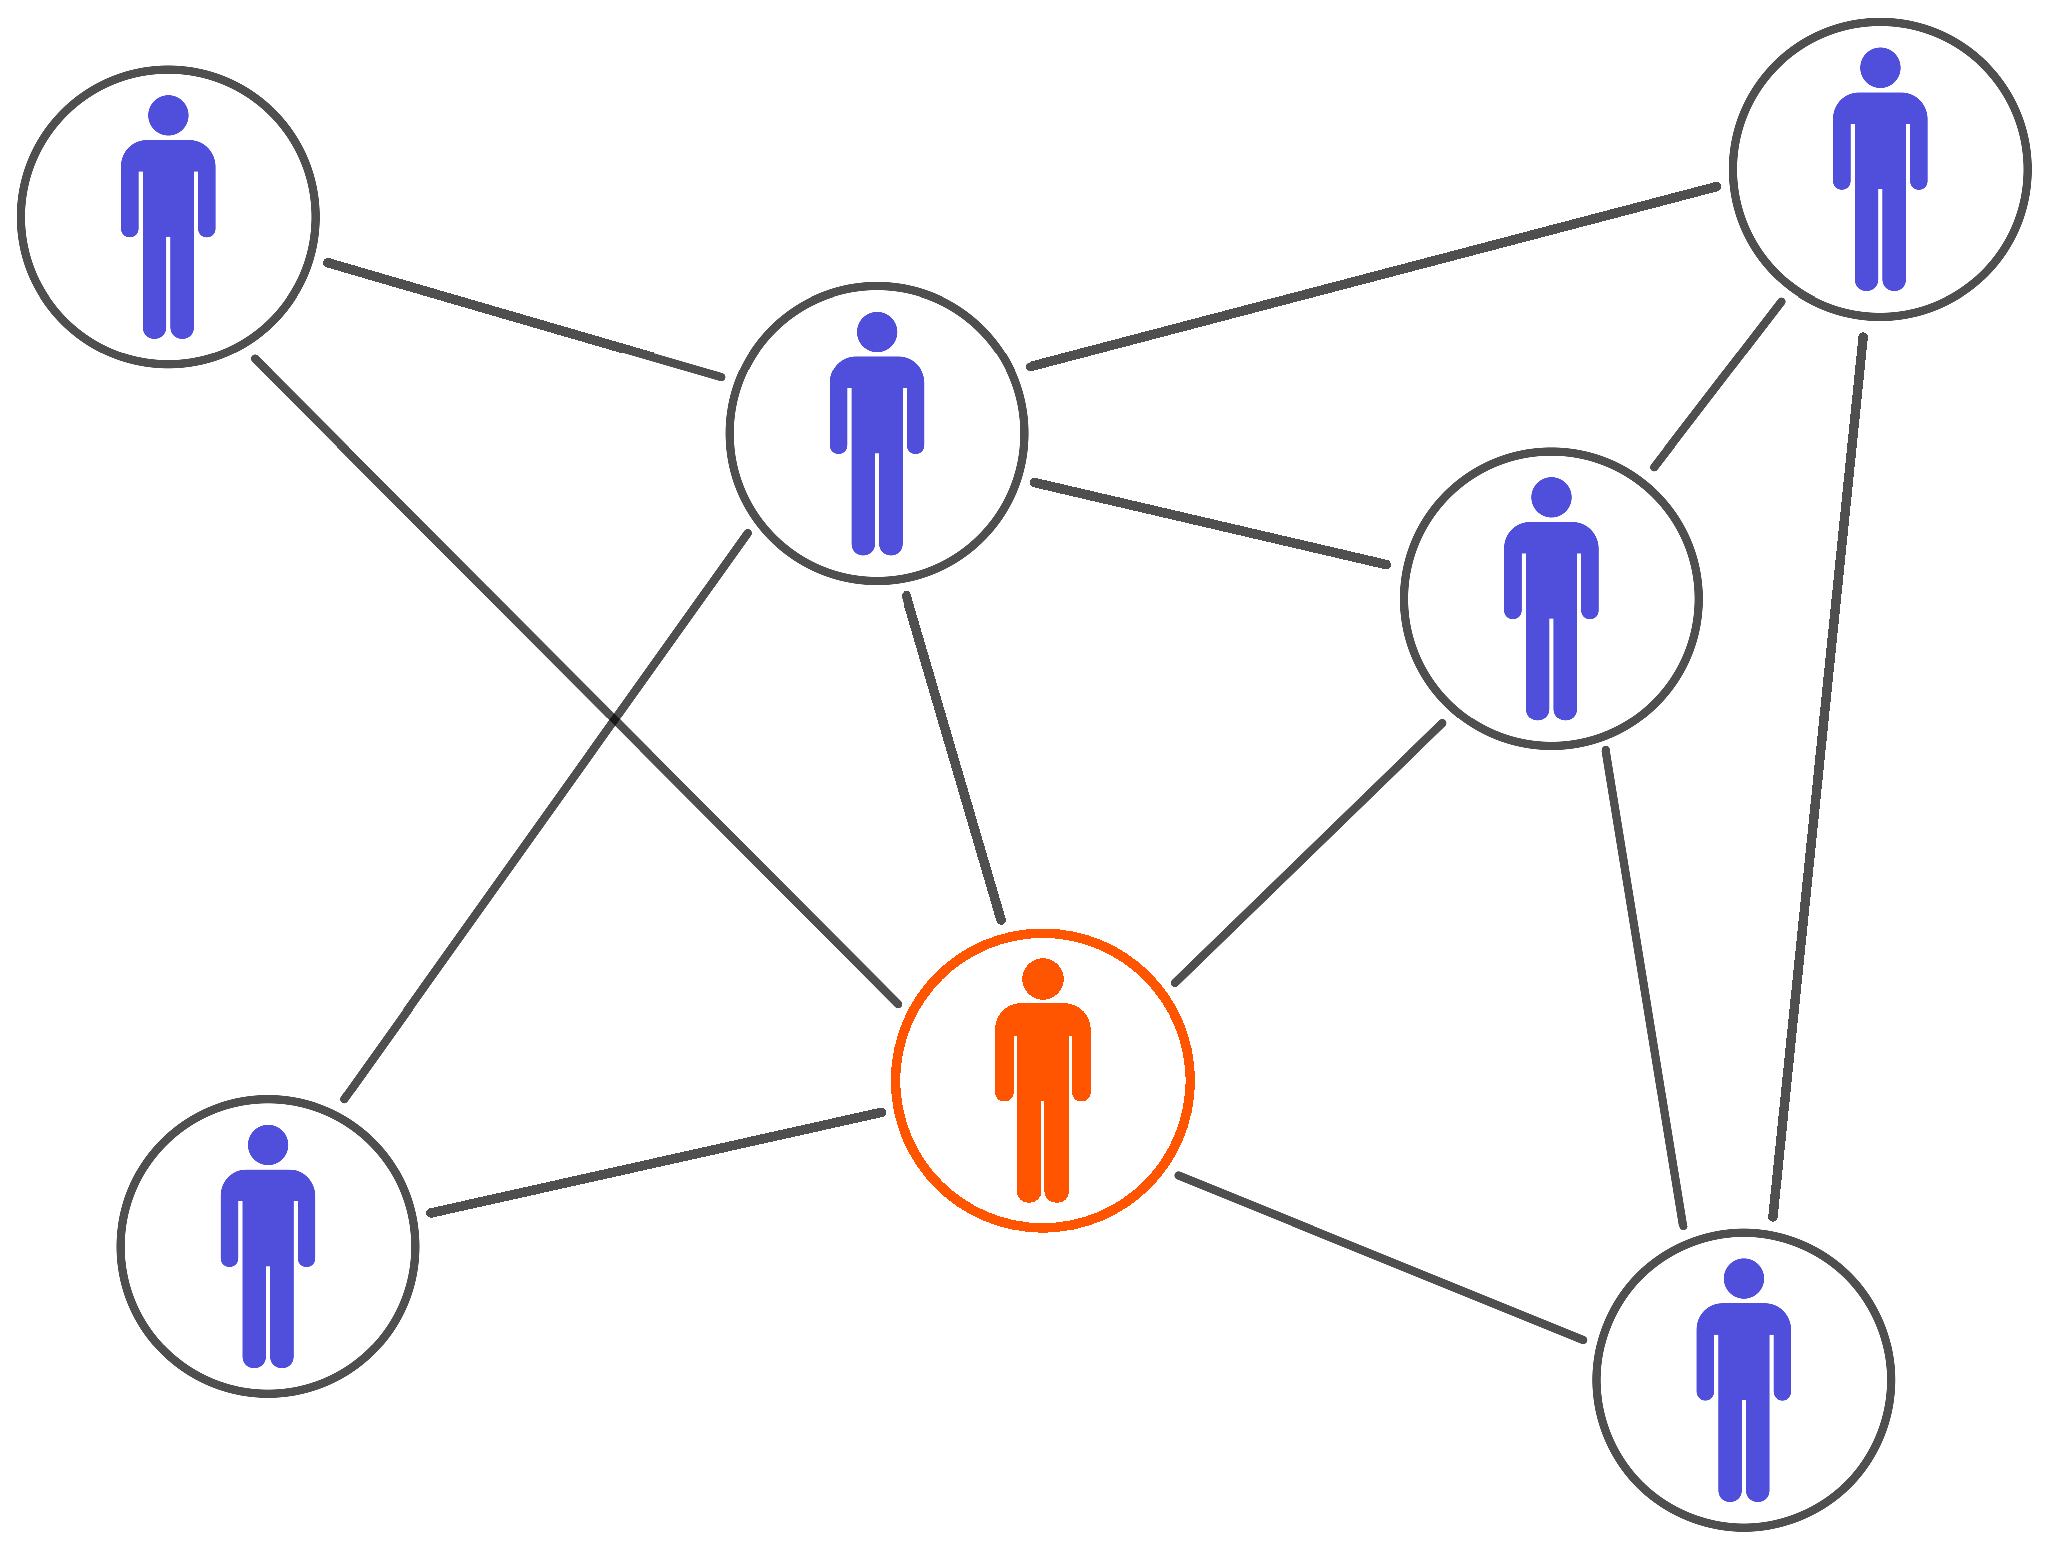
\includegraphics[scale=0.25]{figures/sn1}
 \caption[شبکه‌ی اجتماعی]
 {نمایی کلی از ‌یک شبکه‌ی اجتماعی.}
\end{figure}
\indent
\end{persian}
%\newpage
\subsection{نظریه گراف ‌‌ها}
\begin {persian}
 \noindent
 نظریه‌ی گراف‌ها علاوه بر کاربرد‌‌های فراوانی که در بسیاری از زمینه‌های علمی‌ و مهندسی دارد برای نشان‌دادن و مدل‌سازی ساختار شبکه‌های اجتماعی نیز بکار برده می‌شود.‌ یک شبکه‌ی اجتماعی‌ یک گراف پویاست \cite{easley_networks_2010} که رشد و نمو آن و همین‌طور تشکیل پیوندهای جدید در آن تابعی از زمان است. البته در اکثر اوقات از‌ یک تصویر لحظه‌ای \cite{guille_information_2013} ایستا که ساختار شبکه‌ی اجتماعی مورد نظر را در لحظه‌ی خاصی نشان می‌دهد برای توصیف آن شبکه‌‌‌ اجتماعی استفاده می‌شود. گراف مورد بحث $G=(V,E)$ به صورت مجموعه‌ای از رأس ‌‌ها(گره‌ها) با نام $V$ و مجموعه‌ای از‌ یال‌ها(پیوندها) به‌نام $E=\{ e_{ab}| a,b \in V\}$ نشان داده می‌شود. گراف حاصل می‌تواند جهت‌دار و‌یا بی جهت باشد برای مثال می‌قدرت در توییتر ارتباط‌هایی که دو طرفه می‌باشند، ‌یعنی هر دو طرف توییت‌‌ها و پیام‌های دیگری را دنبال می‌کند به صورت بی جهت در نظر گرفت و ارتباطاتی را که فقط‌ یک طرف دریافت کننده‌ی توییت‌هاست به صورت جهت‌دار نشان داد. همچنین گراف حاصل می‌تواند وزن دار باشد بدین معنا که به هر عضو مجموعه‌ی $E$ عددی را به موضوع وزن به نام $w_
e$ نسبت 
داد. \\
 \indent 
گراف‌های مورد بحث در زمینه شبکه‌‌‌های اجتماعی 
دارای خواص مشترک جالبی مثل کمی‌ فاصله هندسی\پانویس { Geodic distance } بین گره‌ها هستند، \cite{watts_six_2004, boccaletti_complex_2006} که نشان دهنده‌ی پدیده‌ی \lr{Small-world} می‌باشد. هم چنین تعداد‌ یال ‌‌های‌ یک گره تابعی از توزیع‌‌‌های \lr{Heavy-tailed} می‌باشد \cite{boccaletti_complex_2006}.
در جدول صفحه بعد خصوصیت‌های مطرح گراف حاصل از شبکه‌های اجتماعی را مشاهده می‌نمایید.
\\
\begin{table}[H]
%\label{tab:SNGModels}
\centering {
\onehalfspacing
 {\small
 \begin{tabular}{ | l | l | p{4.3cm} |}
 \hline
 {خصوصیت گراف شبکه‌ی اجتماعی} & {رابطه } & {توضیحات} \\ 
 \hline
 
 \lr{power law degree distribution} & $P(x) \sim x^{-\alpha}$ & $P(x)$
 احتمال این را که گره‌ای از $G$ دارای $x$‌یال باشد نشان می‌دهد. ضمنا $\alpha$ عدد ثابتی است که با آزمایش محاسبه می‌شود. \\ \hline
 
 \lr{small-worldness} & $(L = {{\frac{1}{{1 \over 2}n(n-1)}} \sum_{a \geqslant b}{d_{ab}}}) \sim log(n)$ & $L$
 میانگین کوتاه ترین فاصله دو گره دلخواه را نشان می‌دهد که مقدار آن متناسب با تعداد گره‌های گراف شبکه اجتماعی و برابر عدد مثبت کوچکیست. \\ \hline

 \lr{degree centrality} & $C_{D}(v) = \frac{deg(v)}{n-1}$ & $C_{D}(d)$
 نسبت تعداد گره‌های متصل به گره $v$ به کل گره‌ها را نشان می‌دهد. \\ \hline
 
 \lr{closeness centrality(connected graph)} & $C_{C}(v) = \frac{1}{\sum_{t \in (\{V\}-v)}{d_{G}(v,t)}}$ & $C_{C}(v)$
 متوسط طول کوتاه‌ترین مسیر هندسی از گره $v$ تا بقیه گره‌ها را برای گراف همبند $G$ نشان می‌دهد.
 $d_{G}(v,t)$
 طول ‌کوتاه‌ترین مسیر میان دو گره $v$ و $t$ است.
 \\ \hline
 
 \lr{closeness centrality(disconnected graph)} & $C_{C}(v) = \sum_{t \in (\{V\}-v)}{2^{-d_{G}(v,t)}}$ & مانند تعرف قبلی با این تفاوت که برای گراف‌های ناهمبند هم قابل استفاده است.
 \\ \hline
 
 \lr{betweenness centrality} & $C_{B}(v) = \sum_{(s \neq v \neq t) \in \{V\}}{\frac{\sigma_{st}(v)}{\sigma_{st}(*)}}$ & $C_{B}(v)$ برابر مجموع نسبت تعداد کوتاه‌ترین مسیر‌هایی می‌باشد که از گره $v$ می‌گذرند به تعداد کل کوتاه‌ترین مسیر‌های درون یک‌ گراف.
 ضمنا $\sigma_{st}(v)$ تعداد کوتاه‌ترین مسیرهایی که بین دو گره $s$ و $t$ وجود دارند و از گره $v$ می‌گذرند. $\sigma_{st}(*)$ هم تعداد کل کوتاه‌ترین مسیر‌ها مابین دو گره $s$ و $t$ را نشان می‌دهد.
 \\ \hline
 
 \lr{local clustering coefficient(undirected graphs)} & $C_i = \frac{2|\{e_{jk}: v_j,v_k \in N_i, e_{jk} \in E\}|}{k_i(k_i-1)}$ & $C_i$ نشاندهنده‌ی تعداد اتصال‌ها میان همسایگان گره $i$ تقسیم بر کل اتصال‌هایی که همسایگان گره $i$ می‌توانند داشته باشند. $N_i$ مجموعه‌ی همسایگان گره $i$ و $k_i$ تعداد یال‌های متصل به گره $i$ 
 را نشان می‌دهند(برای گراف جهت دار ضریب ۲ در صورت کسر حذف می شود).
 \\ \hline
 
 \lr{global clustering coefficient} & $\bar{C} = \frac{1}{n}\sum_{i=1}^{n} C_i$ & \lr{clustering coefficient} میانگین گراف شبکه‌ی اجتماعی.
 \\ \hline
 
 
 \end{tabular}
 
 
}
\caption{خصوصیات مطرح گراف حاصل از شبکه‌های اجتماعی}
}
\end{table}

\newpage
مدل‌های گرافی متداول و معمول مورد استفاده برای توصیف گراف‌های اجتماعی عبارتند از:

\begin{enumerate}

\item
\lr{Erd\H{o}s–R\'enyi model}\cite{Erdős60onthe}:
اولین مدل توصیف گراف می‌باشد که در سال 1960 ارایه گردید. اسم دیگر این مدل گراف تصادفی است.

\item
\lr{Watts–Strogatz model}\cite{watts1998collective}:
این مدل که در سال ۱۹۹۸ ارایه گردید خصیصه‌ی
\lr{small-worldness} را به خوبی مدل می‌کند.

\item
\lr{Albert–Barab\'asi model}\cite{barabasi1999emergence}:
این مدل در سال ۱۹۹۹ ارایه گردید. خصیصه‌ی بارز این مدل به خوبی مدل‌کردن قانون احتمال توانی وجود گره‌هایی با اتصالات بسیار زیاد در گراف حاصل است. ضمنا این مدل تنها مدل دارای خاصیت رشد است، بدین معنا که تعداد راس‌ها از ابتدا مشخص نیست و به مرور به گراف آغازین بر اساس مفهوم \lr{Preferntial Attachment}(گره‌های جدید تمایل دارند به گره‌هایی که یال‌های بیشتری بدان‌ها متصل هستند متصل شوند.) اضافه می‌شوند. اسم دیگر این مدل، گراف \lr{scale-free} است.

\end{enumerate}

علاوه بر سه مدل مذکور روش‌های دیگری نیز برای تولید گراف‌هایی با خصوصیات شبیه گراف شبکه‌های اجتماعی نیز وجود دارد. برای نمونه گراف‌ حاصل از اعمال ضرب کرونکر\پانویس { \lr{Kronecker product}}\cite{leskovec2010kronecker} و گراف‌های ساخته شده به روش \lr{Forest Fire}\cite{leskovec2005graphs} خصوصیاتی مانند کوچکی فاصله هندسی رئوس به همراه قانون توزیع توانی درجه رأس‌ها را دارا می‌باشند.

\begin{figure}[H]
 \centering
 \includegraphics[scale=0.17]{figures/bcd}
 \caption[بادبادک \lr{K-C}]
 { گرافی که می‌بینید به بادبادک \lr{K-C} معروف است، در این گراف گره‌هایی که بیشترین مقادیر \lr{Centrality} را دارند با حرف اول نوع آن مشخص شده اند.}
\end{figure}

% \begin{table}[H]
% \centering {
% \onehalfspacing
% {\small
% \begin{tabular}{ | l | l | p{4.3cm} |}
% \hline
% 
% {مدل گراف~~~~~~~~} &{رابطه}&{~~~~~~~~توضیحات} \\ 
% \hline
% 
% \lr{Erd\H{o}s–R\'enyi model} & $G(n,p)$ & در این مدل ابتدا $n$ گره تولید می‌شود و با احتمال $p$ در هر گام زمانی $t$ هر گره مثل $a$ در صورت نداشتن اتصال به گرهی مثل $b$ متصل خواهد شد. 
% \\ \hline
% 
% \lr{Watts–Strogatz model} & $G(n,p)$ & در این مدل ابتدا $n$ گره تولید می‌شود و با احتمال $p$ در هر گام زمانی $t$ هر گره مثل $a$ در صورت نداشتن اتصال به گرهی مثل $b$ متصل خواهد شد. 
% \\ \hline
% 
% 
% \end{tabular}
% 
% }
% \caption{خصوصیات مطرح گراف حاصل از شبکه‌های اجتماعی}
% }
% \end{table}


 \begin{figure}[H]
 \centering
 \begin{subfigure}[b]{0.46\textwidth}
 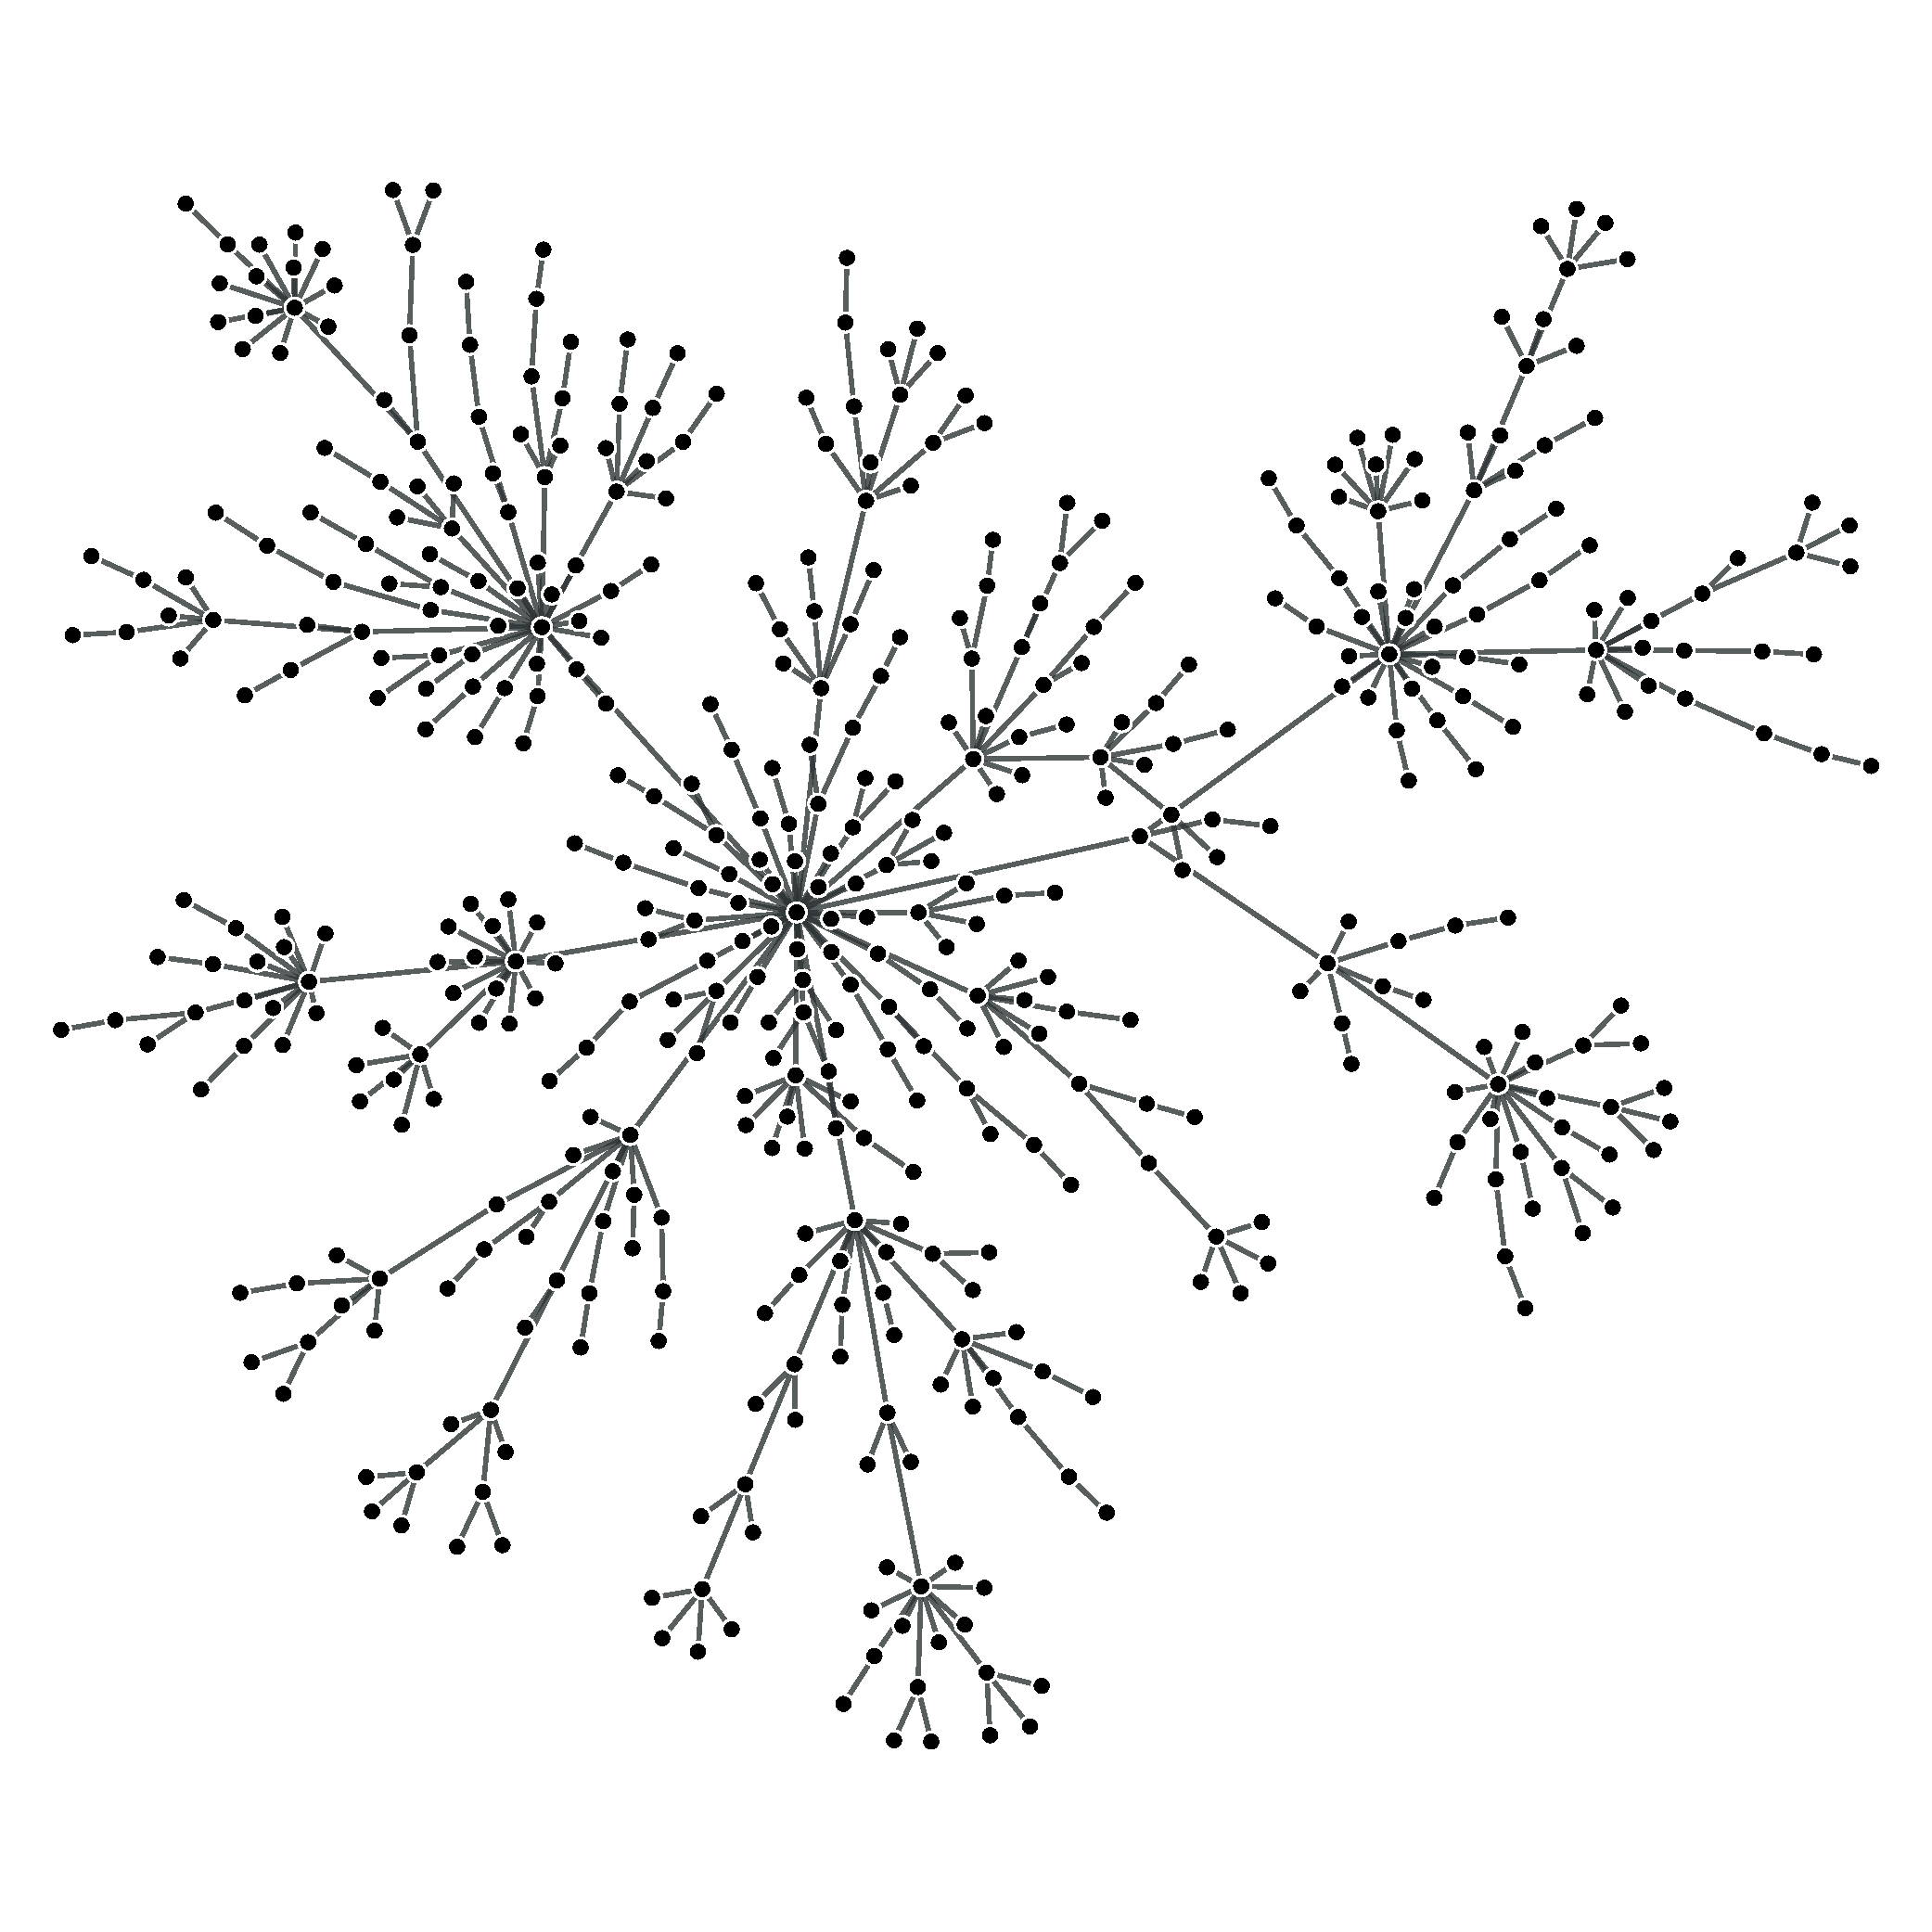
\includegraphics[width=\textwidth]{figures/GRAPHS/power-law}
 \caption{یک گراف با توزیع توانی یال‌ها
 }
 \end{subfigure}
 ~
 \begin{subfigure}[b]{0.4\textwidth}
 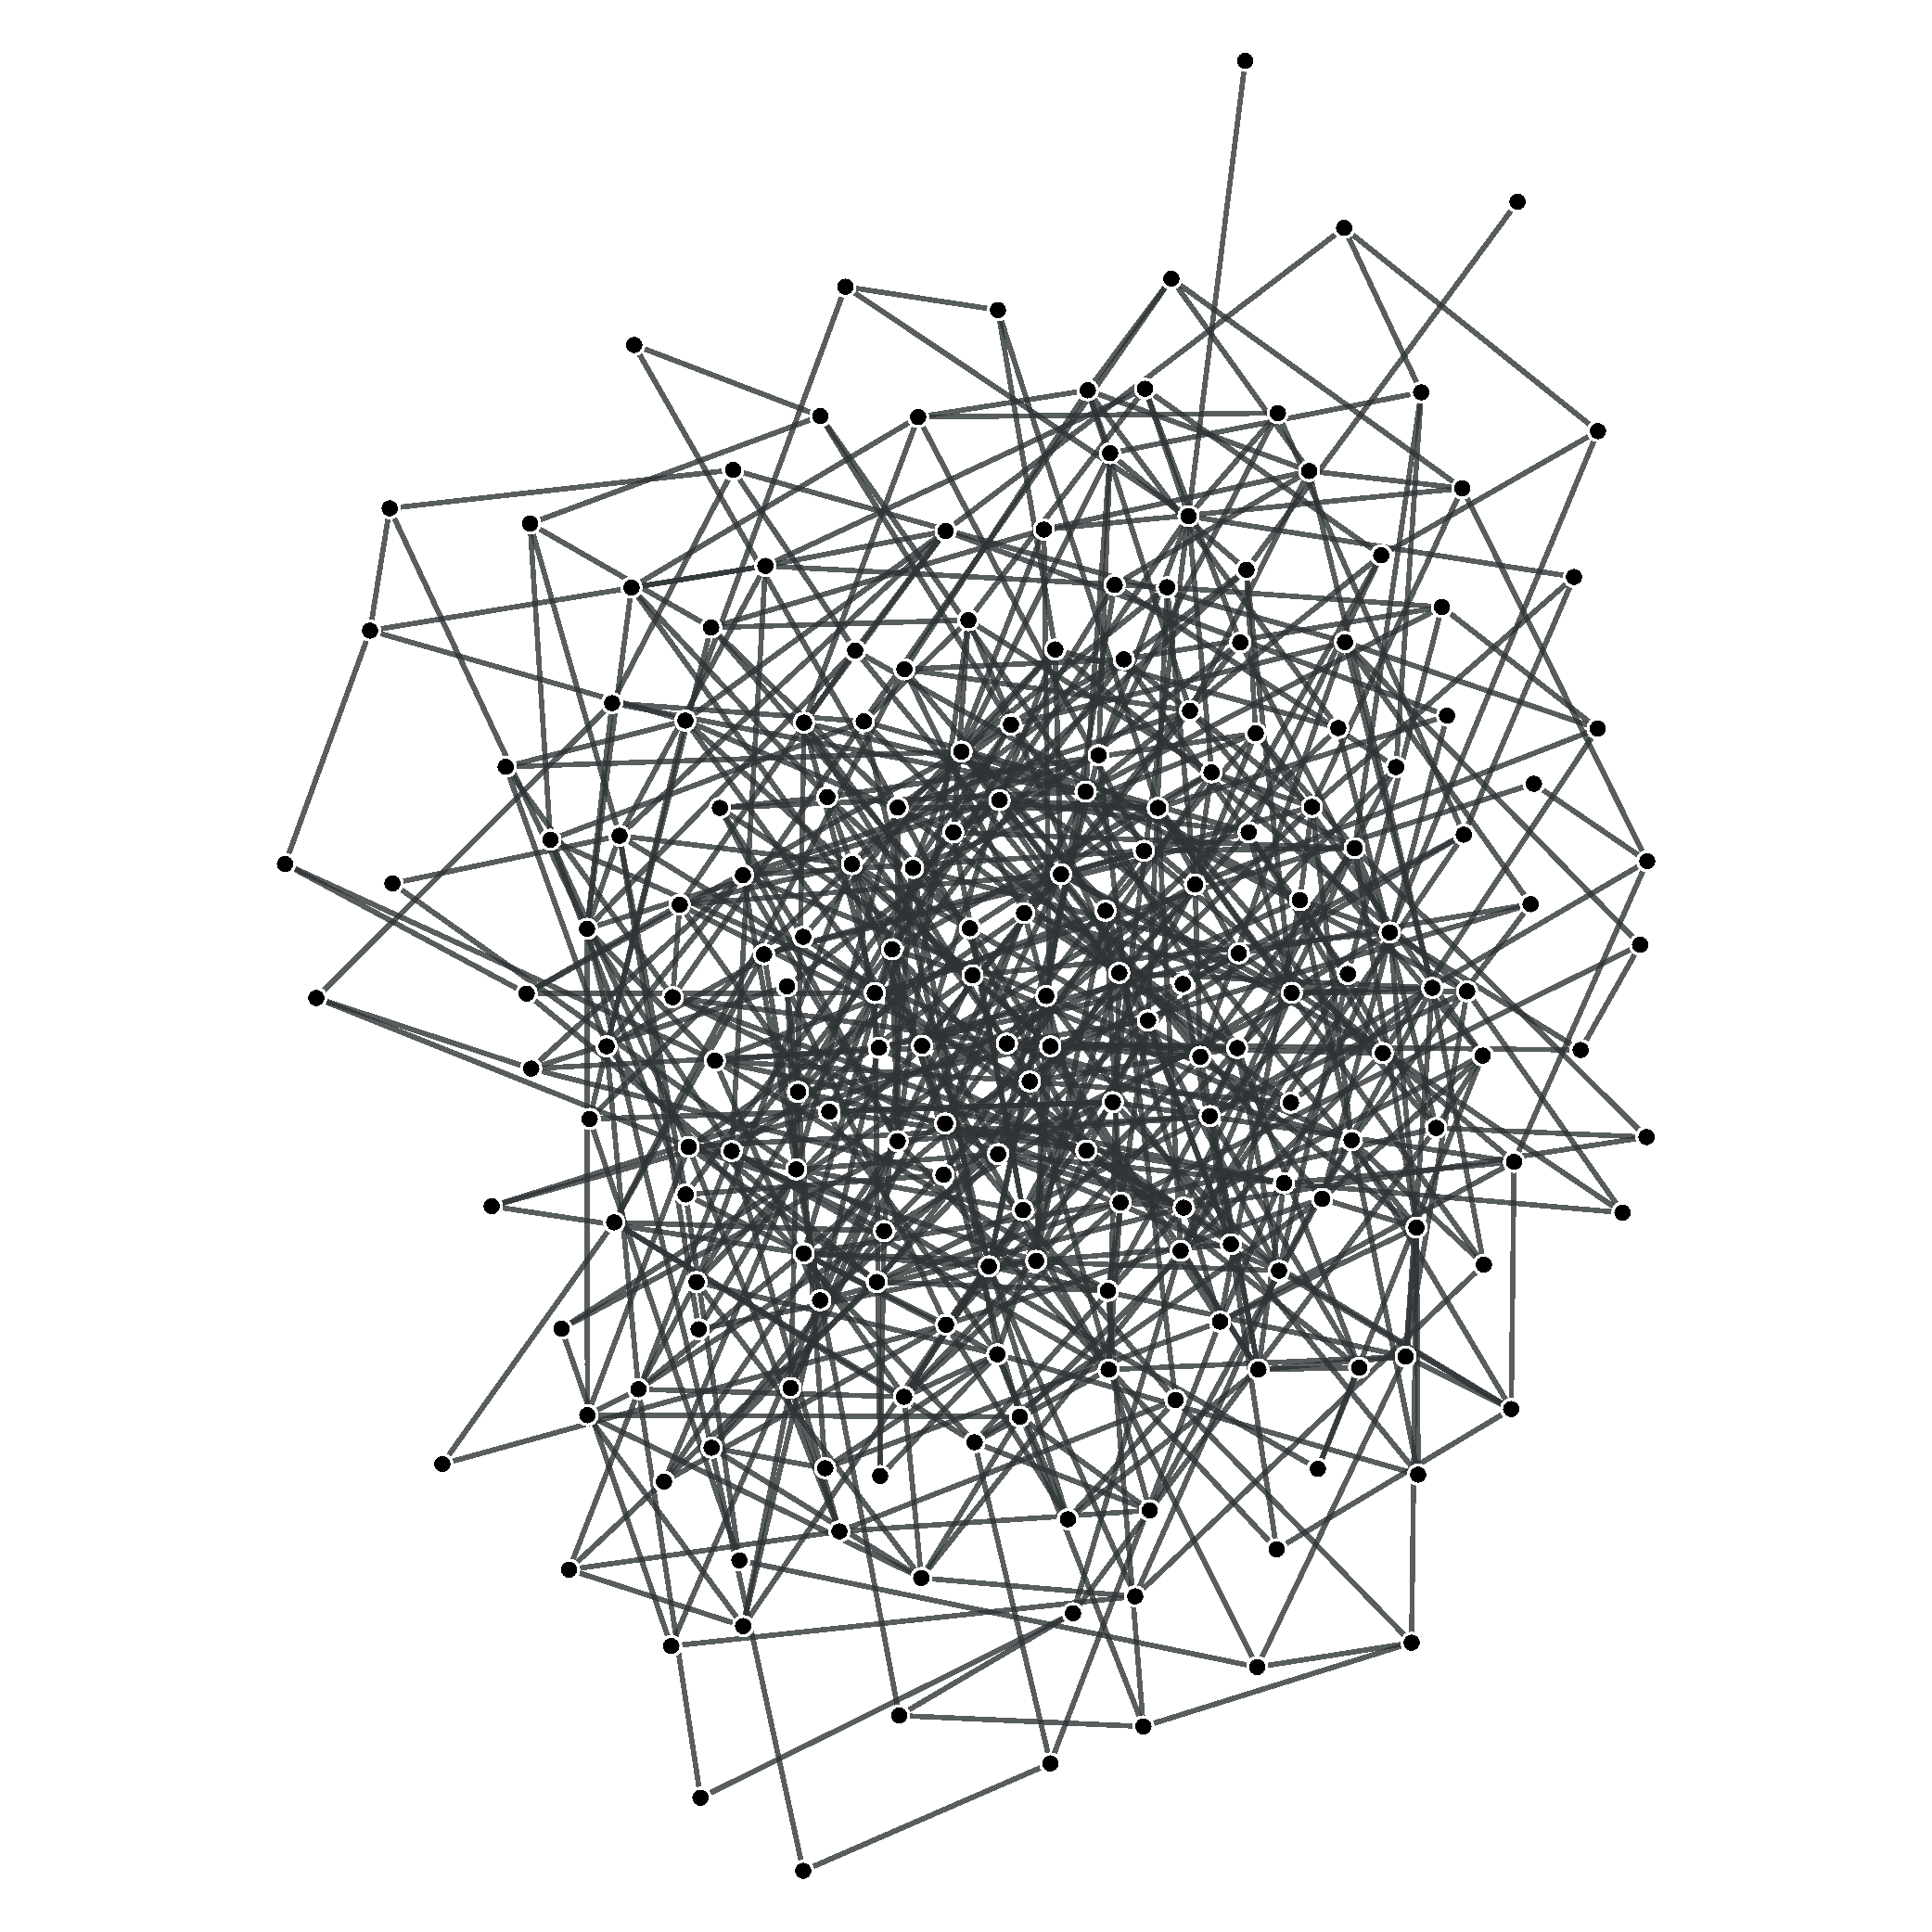
\includegraphics[width=\textwidth]{figures/GRAPHS/small-world}
 \caption{یک گراف \lr{small-world}}
 
 \end{subfigure}
 ~
 \begin{subfigure}[b]{0.58\textwidth}
 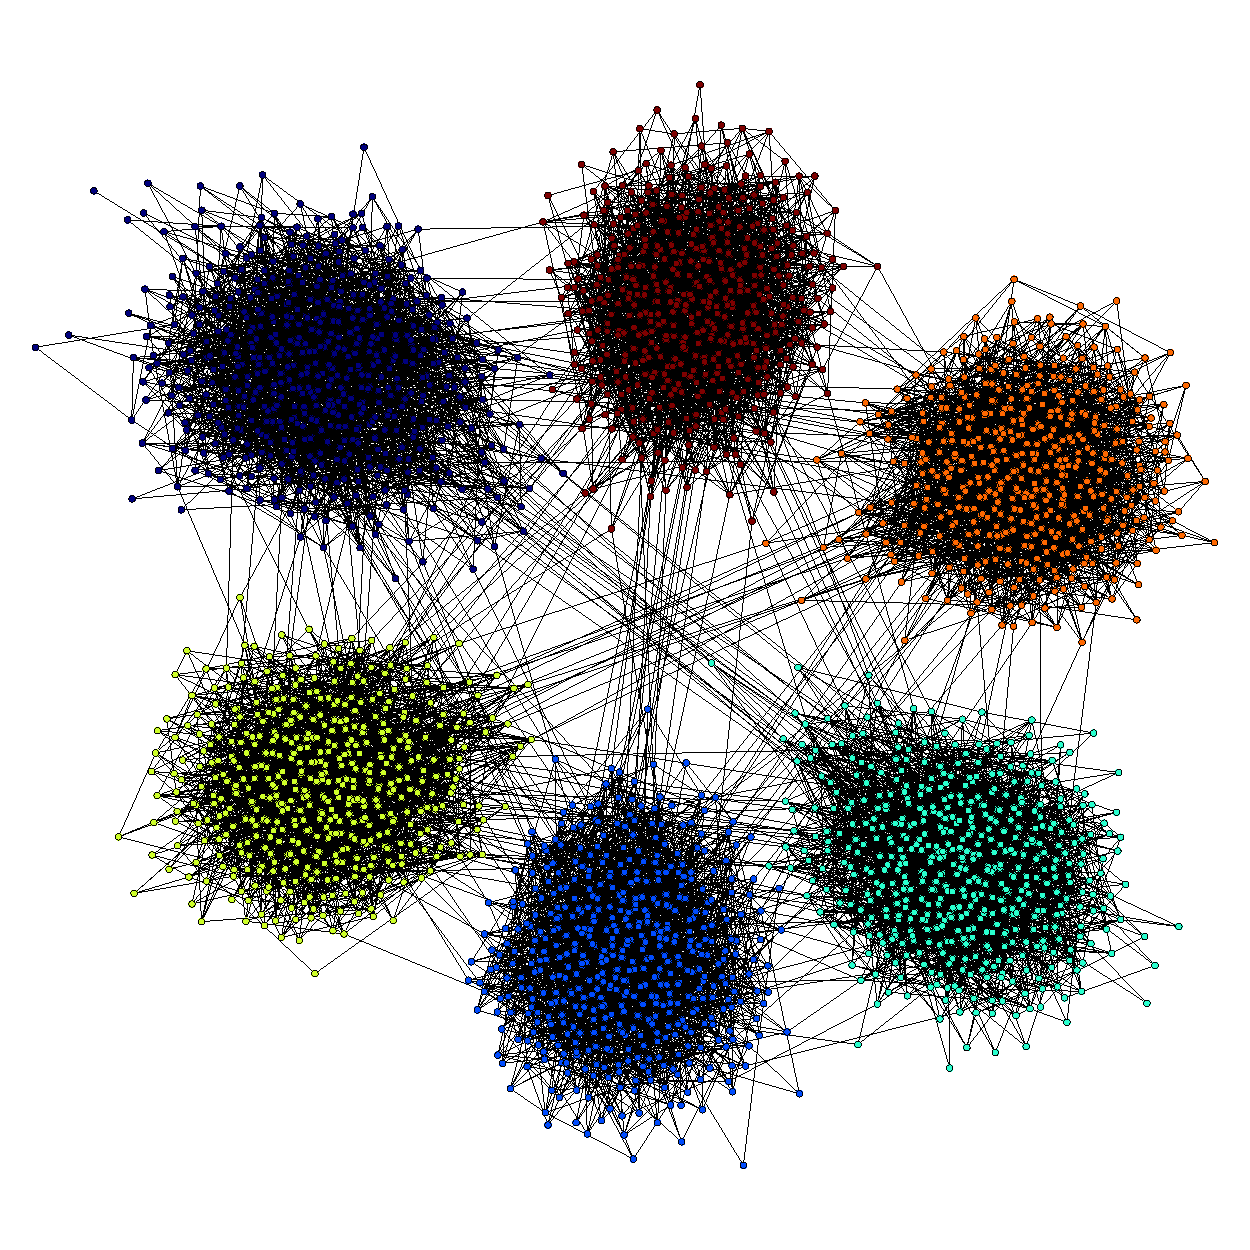
\includegraphics[width=\textwidth]{figures/GRAPHS/clusters}
 \caption{وجود خوشه‌ها‌یی از گره‌ها در گراف شبکه‌های اجتماعی}
 
 \end{subfigure}
 
 \caption[گراف شبکه‌های اجتماعی]{شکل گراف شبکه‌های اجتماعی}
\end{figure}
 
\end {persian}

%\newpage

\subsection{هوموفیلی}

\begin {persian}
\noindent
وجود هوموفیلی\پانویس {\lr{ Homophily}} میان اعضا ‌یکی از خصوصیات بنیادین شبکه‌های اجتماعی می‌باشد. هوموفیلی از طرفی به معنای شباهت ‌یک فرد با افراد مرتبط و همسایگان وی در شبکه‌ی اجتماعی مورد نظر از دید ابعاد مختلف خصوصیتی منتسب بدان فرد مثل سن و علاقه و نژاد می‌باشد \cite{sun_survey_2011}. از طرف دیگر هوموفیلی را می‌قدرت تمایل افراد جامعه به تشکیل رابطه با دیگر اعضای‌ شبیه به خودشان دانست. خصوصیات مورد بحث درباره‌ی هوموفیلی می‌قدرتند قابل تغییر(وزن و علایق) و‌ یا غیر قابل تغییر(نژاد و جنس) باشند \cite{easley_networks_2010}. وجود هوموفیلی میان اعضا به دلیل اینکه مجموعه‌ی همسایگان ‌یک فرد در ‌یک شبکه‌ی اجتماعی‌ یک مجموعه‌ی تصادفی از کل اعضای شبکه‌ی اجتماعی نیست می‌تواند ‌یک نتیجه طبیعی مقایسه‌ی فرد انتخاب شده با همسایگانش باشد \cite{sun_survey_2011}.
سه عامل زیر برای وجود هوموفیلی در شبکه‌های اجتماعی متصوراند \cite{sun_survey_2011}:

\begin{description}

\item[{تاثیر اجتماعی\پانویس {\lr{ Social Influence}}}]{: افراد تمایل دارند مانند دوستان خود رفتار کنند و این امر باعث می‌شود که در‌یک شبکه‌ی اجتماعی افراد رفتارشان تحت تاثیر همسایگانشان باشد.}

\item[انتخاب]{: افراد تمایل دارند با افرادی که از ابتدا به آن ‌‌ها شبیهند همسایه شوند.}
 
\item[متغییر‌های مخفی]{: متغییر‌های دیگری جز دو مورد فوق الذکر که در رفتار افراد جامعه تاثیر گذارند.}
 
\end{description}

 \begin{figure}[H]
 \centering
 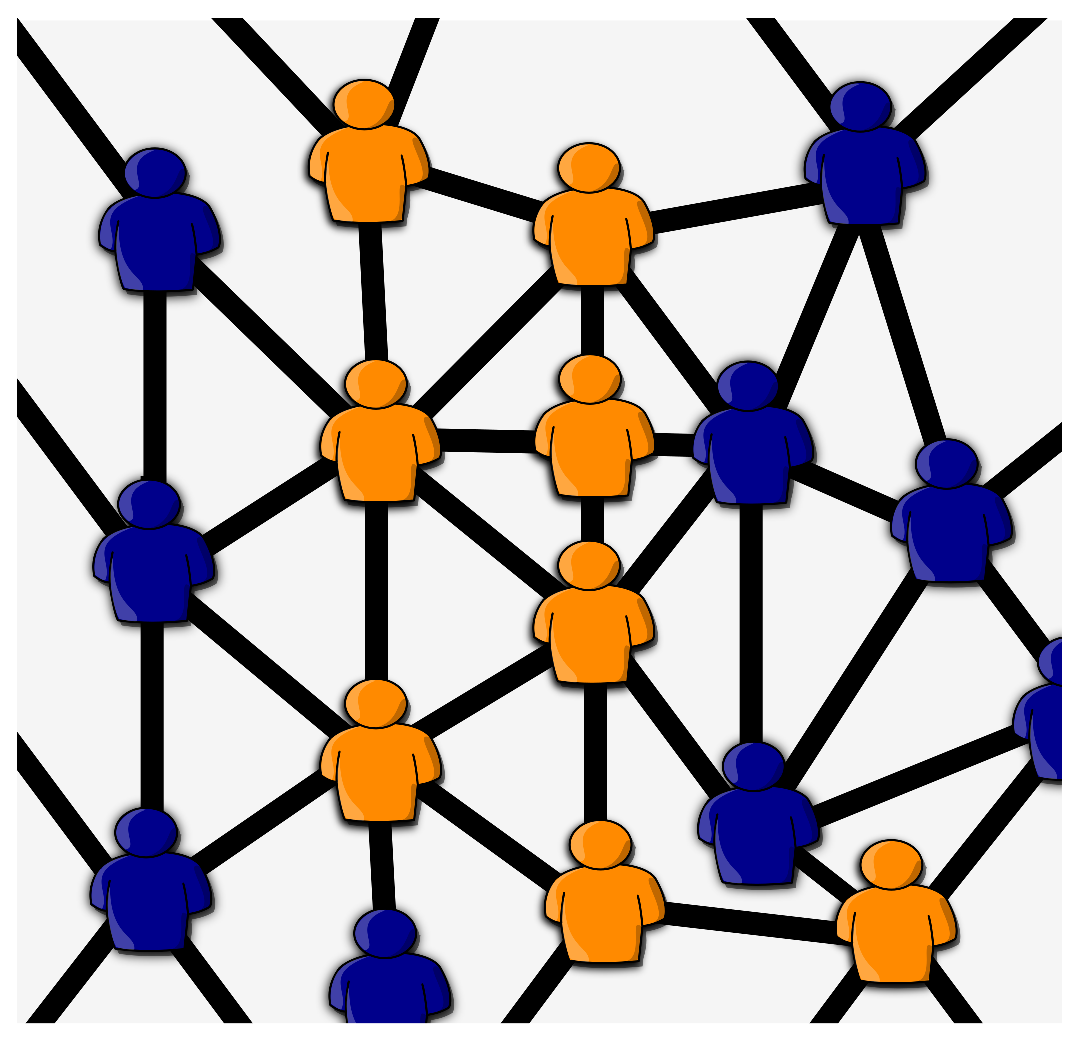
\includegraphics[scale=0.5]{figures/homophily1}
 \caption[هوموفیلی]
 {هوموفیلی: در شبکه‌های اجتماعی اکثر همسایگان و دوستان‌یک فرد دارای صفات شبیه به صفات آن فرد می‌باشند.}
\end{figure}

\indent
مقدار هوموفیلی در‌یک شبکه‌ی اجتماعی‌یک عامل مهم برای بزرگی اندازه‌ی گروه ‌‌هاست \cite{watts_six_2004} به طوری که با فرض اینکه افراد با هوموفیلی بالا معمولا تمایل زیادی با برقراری رابطه تنها با افراد شبیه به خودشان دارند، در این صورت هوموفیلی زیاد نشان دهنده‌ی گروه‌های کوچک تر و کوچکی میزان هوموفیلی نشان دهنده‌ی وجود گوناگونی در صفات همسایگان در ‌یک شبکه‌ی اجتماعی است. از طرفی‌ یکی از پیامد‌‌های پدیده‌ی پخش‌اطلاعات و نمود‌های سطح بالای آن تاثیر آن در رفتار اعضا می‌باشد. هوموفیلی به موضوع‌ یکی از موارد دخیل در شکل‌گیری و نمو گراف ساختار شبکه‌ی‌های اجتماعی که فرایند پخش اطلاعات روی آن ‌‌ها صورت می‌پذیرد مورد توجه پژوهش گران در زمینه‌ی پدیده‌ی پخش اطلاعات می‌باشد \cite{weng_role_2013}. 

\end {persian}

%\newpage
\subsection{فرضیه قدرت اتصال‌های ضعیف}
\begin {persian}
\noindent
مارک گرانوتر در سال ۱۹۷۳ نظریه قدرت اتصال‌های ضعیف\پانویس{ Strength of Weak Ties} \cite{granovetter_strength_1973} را مطرح نمود که ‌یکی از پیامد‌های آن تاکید بر تاثیری می‌باشد که اتصال‌های ضعیف و به عبارتی پل ‌‌ها\پانویس { Bridge } در گراف شبکه‌های اجتماعی در انتقال اطلاعات و تسهیل امکان ارتباط میان زیرجوامع\پانویس{ Sub-Community} جدا از هم بازی می‌کنند.\\
\indent
به زبان ساده تر بر اساس این نظریه اتصال‌های ضعیف (برای نمونه پل ‌‌ها) با اینکه قادر به انتقال حجم زیادی از اطلاعات نیستند باز نقش مهمی‌در جابجایی نوآوری و اطلاعات نوع در سطح شبکه‌های اجتماعی ایفا می‌کنند. از طرفی وجود اتصال‌های ضعیف زیاد می‌تواند به کندی فرایند پخش بیانجامد \cite{guille_information_2013,sun_survey_2011}. هم چنین بر طبق قدرت اتصال‌های اجتماعی با تعداد تکرار آن اتصال در دایره‌های اجتماعی اعضا رابطه دارد.
 \begin{figure}[H]
 \centering
 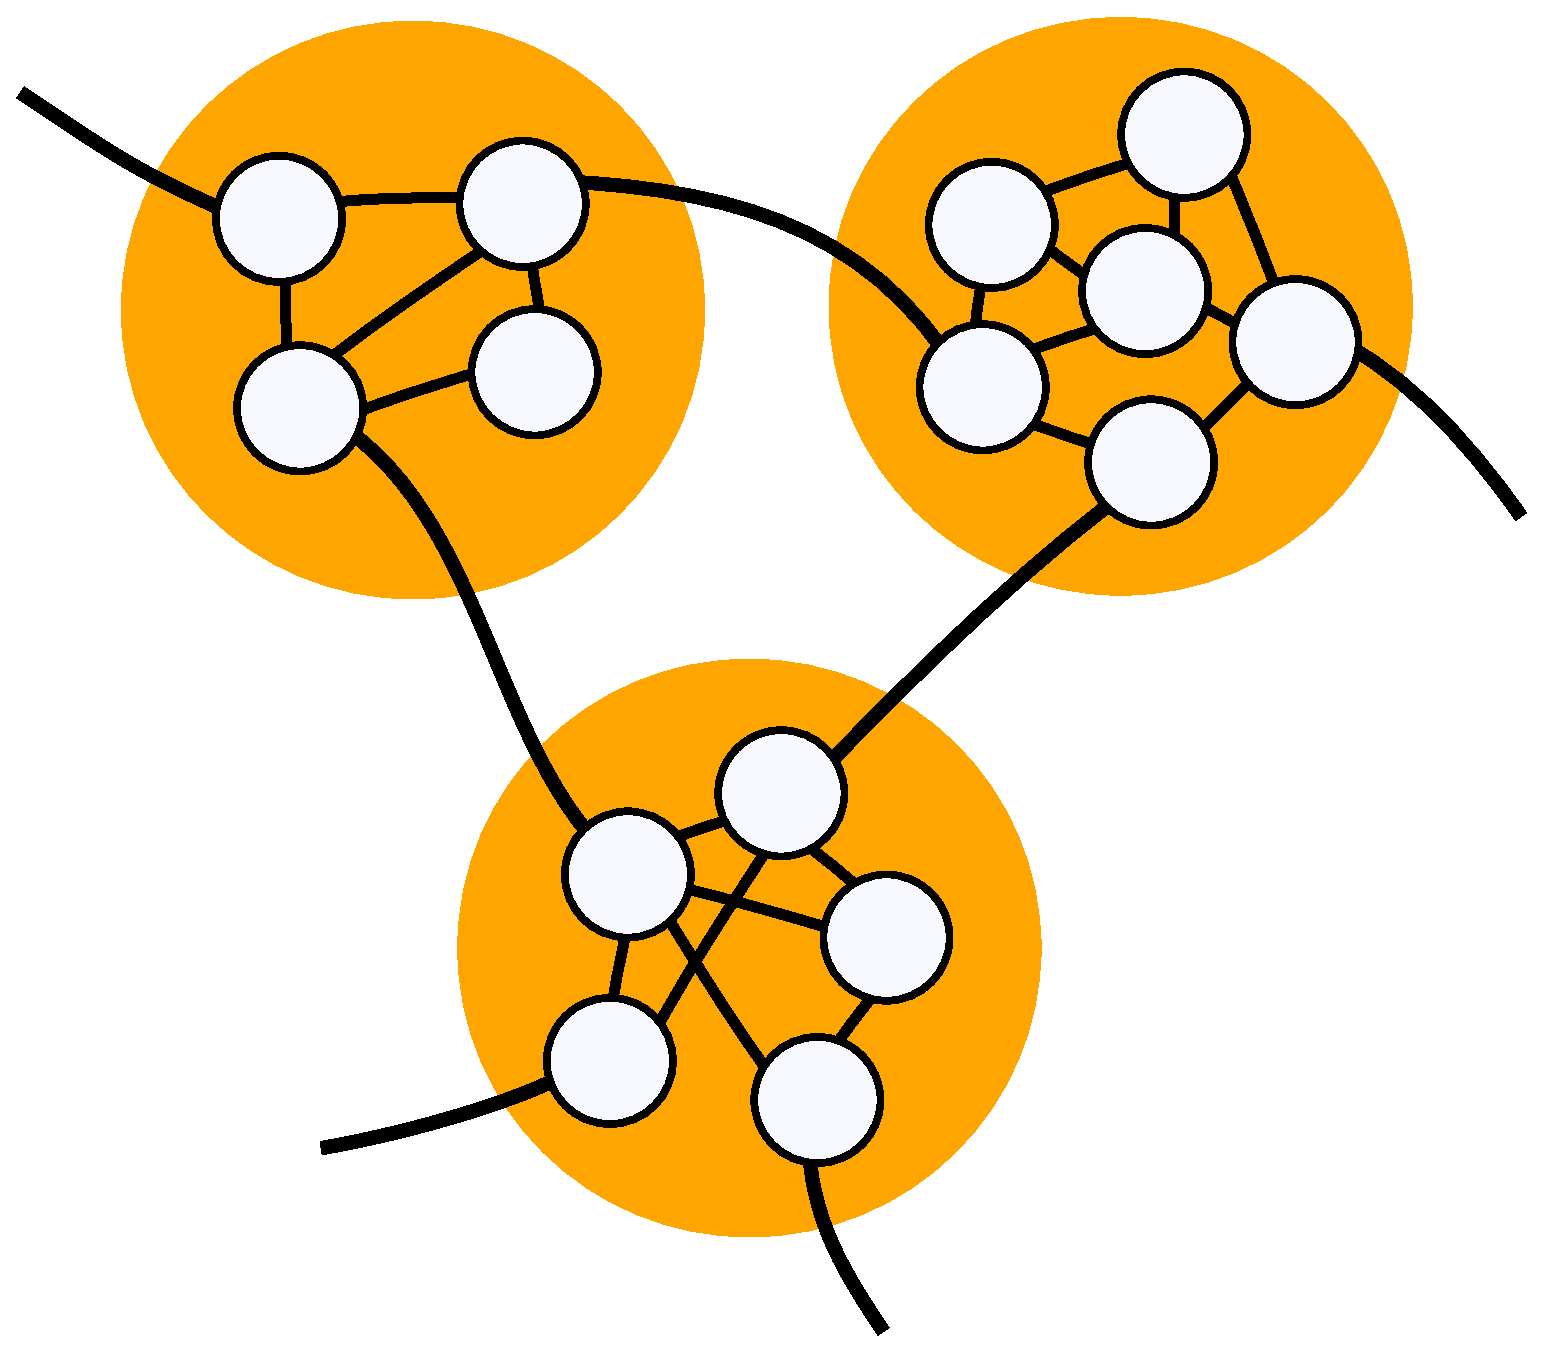
\includegraphics[scale=0.29]{figures/swt}
 \caption[فرضیه قدرت‌های ضعیف]
 {نمایی از اتصال‌های قوی(نازک تر) و ضعیف(کلفت تر) میان اعضا.}
\end{figure}


قدرت اتصال‌ها میان گره‌ها در یک شبکه‌ی اجتماعی که به صورت یک گراف مدل شده است به صورت زیر تعریف می شود.
\begin{center}
%\scalebox{1.25}
 { $ Strength_{ab} = \frac{ N(a,b) }{d(a)-1 ~+~ d(b)-1 ~-~N(a,b) } $}

\end{center}
در این فرمول $N(a,b)$ نشانده‌ی همسایه‌های مشترک گره‌های $a$ و $b$ است. $d(x)$ هم نشاندهنده‌ی تعداد یال‌های متصل به گره $x$ می باشد. برای یک گراف بی‌جهت $Strength_{ba} = Strength_{ab}$ خواهد بود.

\end{persian}

\section{فرایند پخش اطلاعات}
\begin {persian}
\noindent
فرایند پخش شدن اطلاعات به جابه جایی اطلاعات(دانش) از فردی به فرد دیگر در‌یک شبکه‌ی اجتماعی و ارتباطی اطلاق می‌شود \cite{zafarani_social_2014}. این فرایند با درنظر گرفتن زیرساخت یک شبکه‌ی اجتماعی که معمولا با یک گراف ایستا نمایش داده می شود، دارای اجزای اصلی زیر است \cite{wu_dynamics_2013}:
\begin{description}

\item[افراد]{کسانی که محتوا را تولید و مصرف می‌کنند.}

\item[محتوا]{انواع مختلف اطلاعات مثل خبر و توییت و عکس.}
 
\item[شبکه ارتباطات]{شبکه‌ی زیرین افراد و روابط آن ‌‌ها که تحت تاثیر فرایند پخش اطلاعات قرار دارد و همین طور ساختار آن این فرایند را تحت تاثیر قرار می‌دهد.}
 
\end{description}
 \begin{figure}[H]
 \centering
 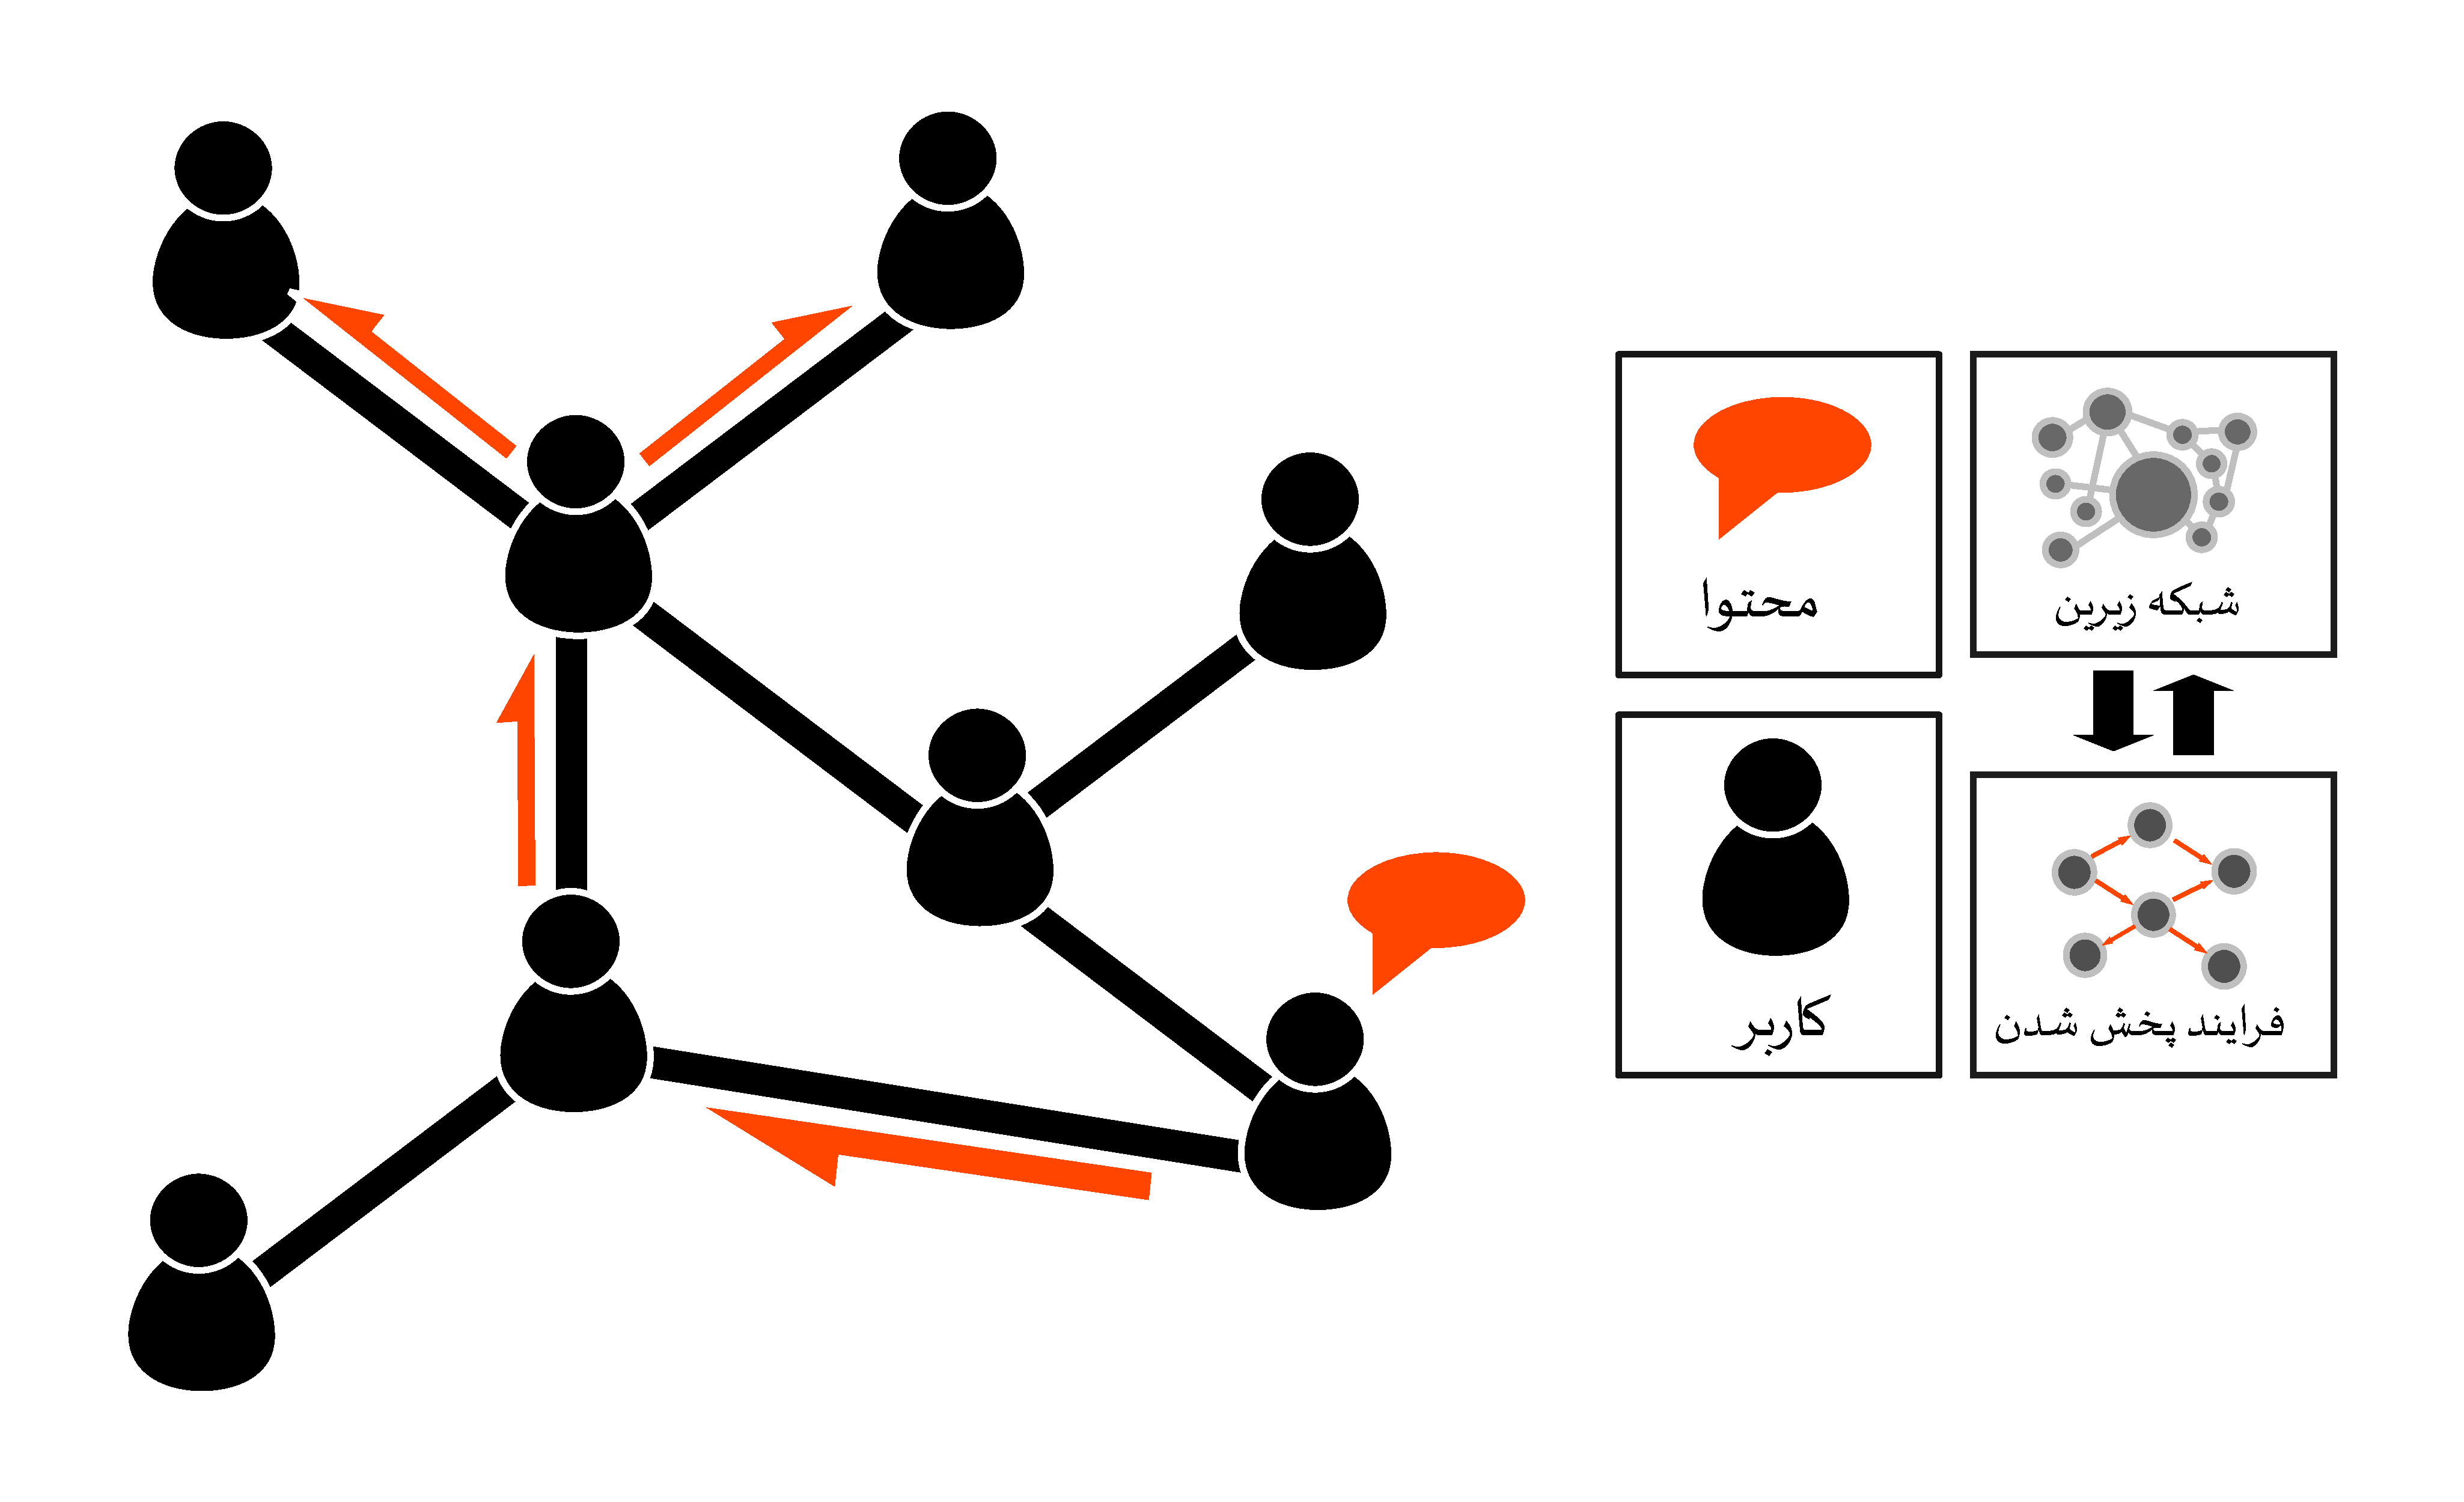
\includegraphics[scale=0.23]{figures/diffusion1}
 \caption[فرایند پخش اطلاعات در ‌یک گراف]
 {نمایی کلی از فرایند پخش اطلاعات در ‌یک گراف شبکه‌ی اجتماعی.}
\end{figure}

البته اجزای این فرایند در \cite{zafarani_social_2014} به صورتی سطح بالاتر به شکل زیر تعریف شده است:
\begin{description}

\item[فرستنده‌ها]{مجموعه‌ای معمولا کوچک از افراد که امر پخش با آن‌ها شروع می شود.}

\item[گیرنده‌ها]{مجموعه‌ای از افراد با جمعیتی بسیار زیادتر از فرستنده‌ها که محتوای فرستنده‌ها را دریافت می‌کنند.}
 
\item[ظرف]{ظرفی که محتوای اطلاعاتی مورد تبادل می‌شود. برای مثال پیام‌های یک کاربر در فیسبوک که توسط دوستانش دیده می‌شود.}

اطلاعات مورد بحث در اینجا می قدرتد یکی از موارد \textbf{شایعه} یا بکارگیری یک \textbf{تکنولوژی نوین} و یا یک \textbf{خبر} و حتی یک \textbf{تاثیر اجتماعی} که در حال فراگیری و پخش در سطح شبکه‌ی اجتماعی است باشد.
\end{description}

 \begin{figure}[H]
 \centering
 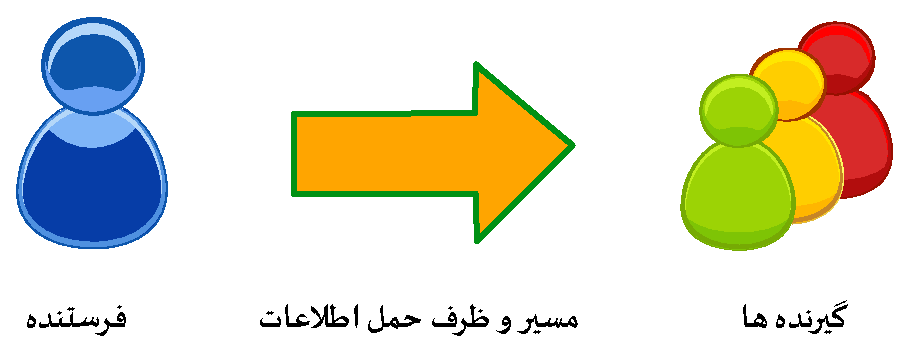
\includegraphics[scale=0.55]{figures/Diff}
 \caption[ دید کلی از فرایند پخش‌ اطلاعات]
 {نمایی کلی از پخش اطلاعات به صورت عمومی.}
\end{figure}


\end {persian}

\section{یافتن و ردیابی موضوعات مورد توجه در پخش‌اطلاعات}
\noindent {
ردیابی و شناسایی موضوعات مورد توجه در سایت‌های اجتماعی آنلاین و به طور عام سایت‌های خبری و میکروبلاگینگ\پانویس { Microblogging} مثل ارکوت\پانویس{Orkut } و توییتر معمولا در قالب شناسایی نوع موضوع شناسایی شده انجام می‌شود \cite {takahashi_discovering_2011}. 
}

\subsection{موضوع متنی}
\noindent {
در یک شبکه‌ی اجتماعی یک موضوع متنی عبارت است از یک مجموعه از عبارات مرتبط از لحاظ معنای کل که به یک مفهوم مشترک اشاره دارد \cite{guille_information_2013}.
\\
\indent
طبق این تعریف عبارت موضوع برای محتوای پیام‌های متنی تعریف شده است. از طرفی می‌قدرت این تعریف را به سه گونه تفسیر کرد:
\begin{itemize}
 \item [\textbf{الف}]
 {مجموعه‌ای از عبارات به نام $S$ و $|S|=1$}
 \item [\textbf{ب}]
 {مجموعه‌ای از عبارات به نام $S$ و $|S|>1$}
 \item [\textbf{ج}]
 {مجموعه‌ای از عبارات به نام $S$ و توزیع احتمال عبارات موجود در $S$}
\end{itemize}


}

\indent
البته باید در این جا باید متذکر شویم که فرض ما در ادامه‌ی این فصل بر این خواهد بود که منظور از عبارت موضوع همان موضوع محتوای متنی می باشد، و هر نوع موضوع مورد بحثی از این نوع است.
 \begin{figure}[H]
 \centering
 \includegraphics[scale=0.6]{figures/TOPIC}
 \caption[پیام‌های در چرخش]
 {نمایی از چرخش پیام‌ها مابین کاربران \cite{guille_information_2013}.}
\end{figure}

\subsection{موضوع‌های انفجاری}
\noindent {
موضوع‌های انفجاری\پانویس { Bursty Topics} به موضوع‌های خبری گفته می‌شود در بازه‌ی زمانی مشخصی روی رفتار کاربران سایت‌های اجتماعی تاثیر می‌گذارند و این تاثیر قابل رصد می‌باشد. خاصیت اصلی این موضوعات محدود بودن مدت زمان تاثیر آن‌ها به بازه‌ی مورد بحث است به طوری که پیش از شروع زمان بازه و همین گونه پس از آن اثری از رابطه‌ی موضوع و تاثیر آن زیاد به چشم نمی‌آید \cite{guille_information_2013}. همه‌‌ی کار‌های انجام گرفته در این زمینه درباره‌ی شناسایی و ردیابی موضوعات برای داده‌ی متنی محض می باشد.
\\
%\indent

 \begin{figure}[H]
 \centering
 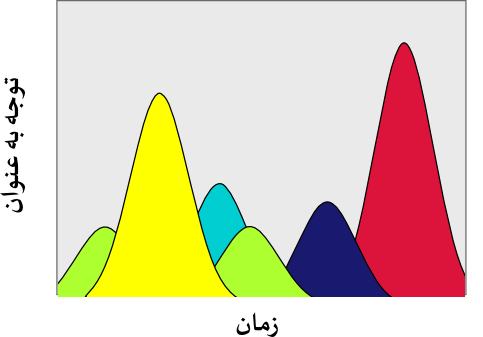
\includegraphics[scale=0.6]{figures/others/BT}
 \caption[موضوع‌های مهم]
 {نمایی از میزان توجه به موضوعات مهم که فرایندی انفجاری را نشان می دهد \cite{guille_information_2013}.}
\end{figure}

 \begin{figure}[H]
 \centering
 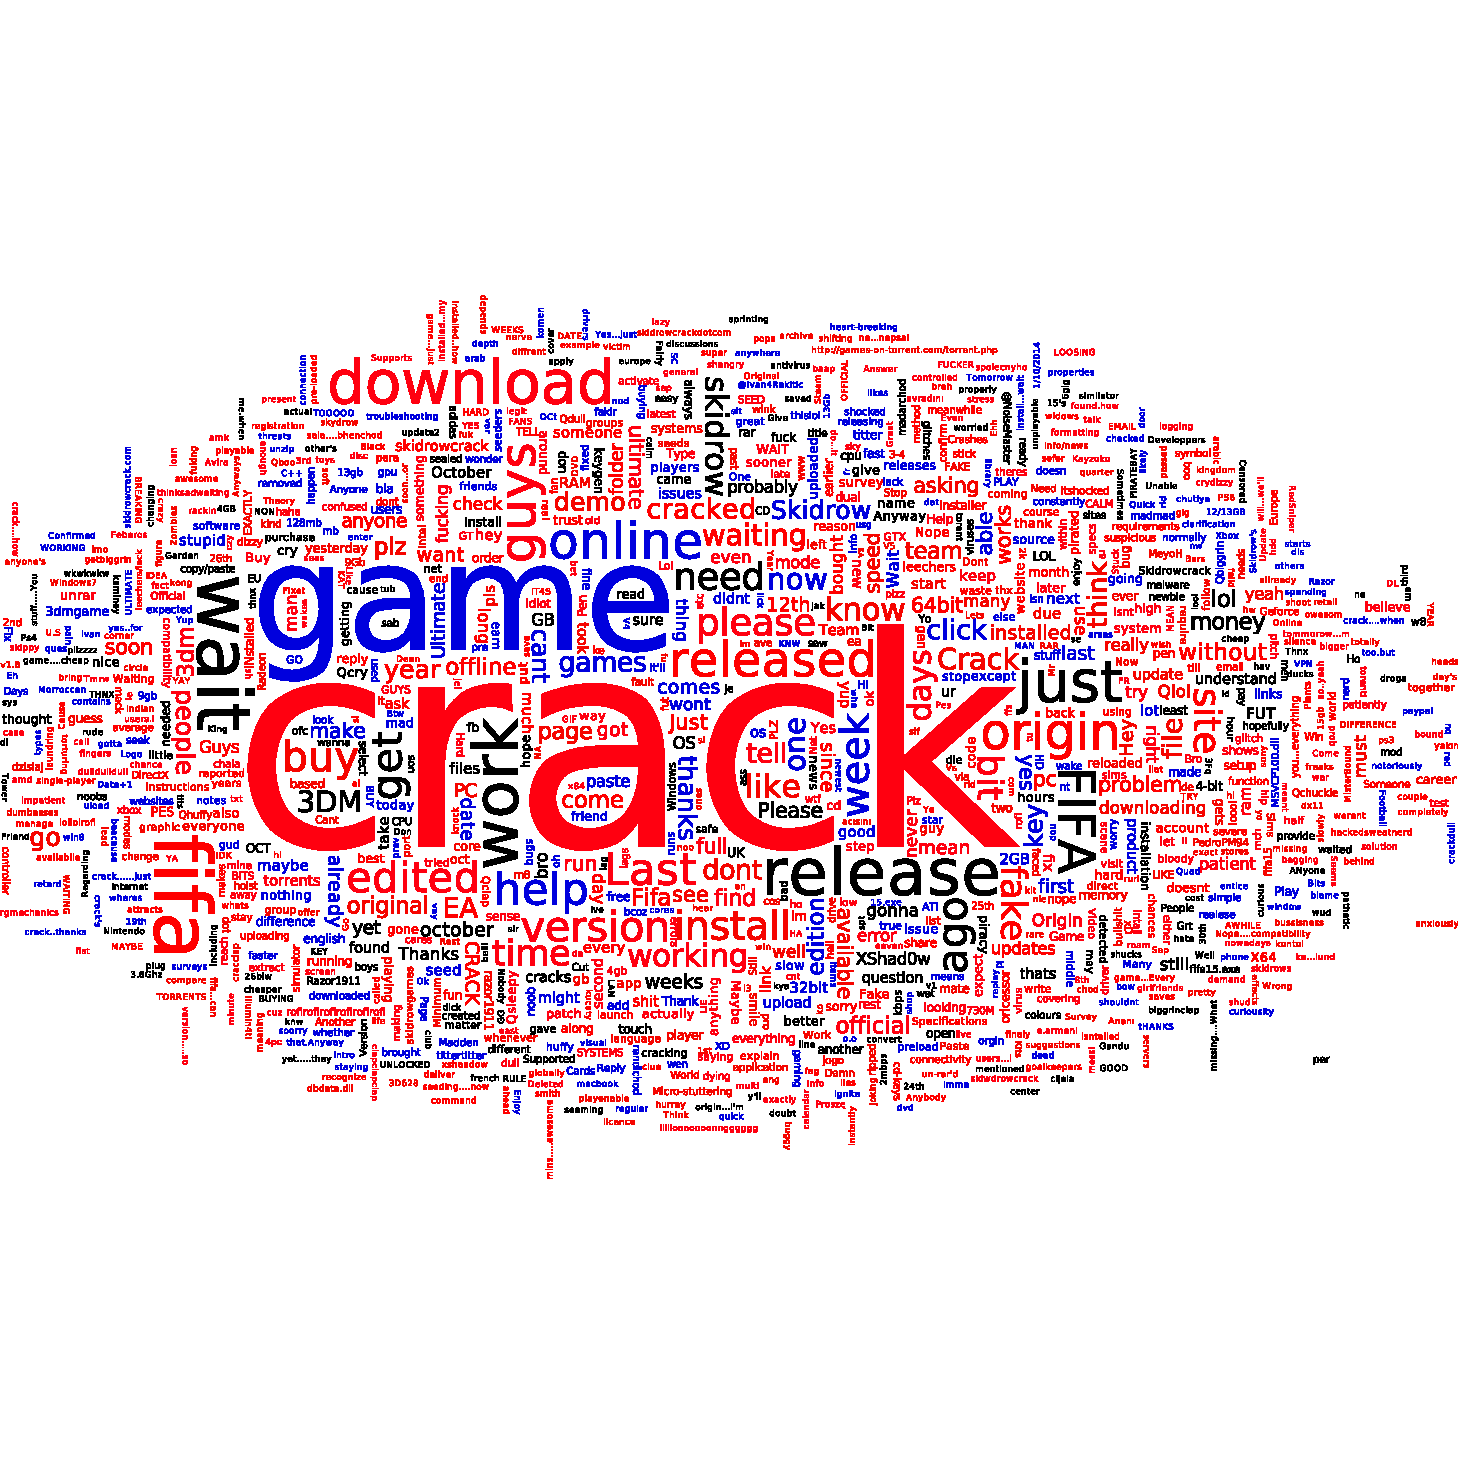
\includegraphics[scale=0.5]{figures/others/fifa15}
 \caption[خبر انتشار بازی میان کاربران سایت تورنت]
 {نمایی از \lr{WordCloud} کلماتی که کاربران سایت
 \href{https://kickass.to/fifa-15-ultimate-team-edition-sc-t9600660.html\#comment}{\lr{KickAss.to}}
 با هم درباره‌ی بازی \lr{Fifa 15} از تاریخ ۱۸ سپتامبر تا ۵ اکتبر ۲۰۱۴ رد و بدل نموده اند.
 }
\end{figure}


}

\section{ محدودیت در توجه و اقتصاد توجه}
\begin {persian}
\noindent
بر طبق نظریه دانبر \cite{dunbar_social_1998}‌یک انسان امروزی قادر به برقراری رابطه اجتماعی پایدار با تعداد معدودی از دیگر اعضای جامعه می‌باشد. از طرفی بر طبق نظریه اقتصاد توجه که توسط سیمون \cite{lilian_weng_information_2014,simon_designing_1971} مطرح شده است حجم زیاد اطلاعات نیازمند(همان مقدار) توجه می‌باشد، حجم این اطلاعات(موجود در شبکه‌های اجتماعی آنلاین) بسیار بیشتر از قدرت توجه و دریافت افراد این جوامع می‌باشد. برای نمونه شبکه‌های اجتماعی آنلاین مانند توییتر که کاربران آن داده‌های بسیار زیاد و متنوعی را در قالب پیام‌های بسیار فشرده تولید می‌کنند.‌ یکی از موارد مهمی‌ که از دو مورد مطرح شده برداشت می‌شود وجود محدودیت برای توجه به محتوای موجود در سایتی مثل توییتر است. چنین فرضی در مطالعه چگونگی فرایند پخش اطلاعات در سطح شبکه‌های اجتماعی آنلاین مورد توجه می‌باشد.

\end{persian}


\section{میم}
\begin {persian}
\noindent
میم\پانویس { Meme } به معنی ایده و‌ یا رفتار و‌ یا همین‌گونه منشی است که در‌ یک فرهنگ از فردی به فرد دیگر قابل انتقال و سرایت است \cite{blackmore_meme_2000}، به زبان ساده تر همان گونه که ژن‌ها واحد انتقال خصایص ‌یک موجود زنده به فرزندانش هستند میم هم واحد انتقال مفاهیم و ایده‌‌ها و رفتارها در فرهنگ‌های حاکم در جوامع انسانی می‌باشد. ریچارد داکینز اولین بار این مفهوم را در کنار مفهوم تکامل و انتقال خواص ژنتیک از نسلی به نسل بعد به خاطر شباهت بین این دو مورد، به کار برده است \cite{dawkins_selfish_1976}. 
\\
\indent
با توجه به گوناگونی زیاد نوع‌های رسانه‌های آنلاین و نیاز‌ به مفهومی‌ خنثی از محتوای رسانه‌های اجتماعی آنلاین میم در تحقیق در زمینه‌های چگونگی انتشار و پخش افکار و اطلاعات در سطح شبکه‌های اجتماعی آنلاین مورد توجه می‌باشد، برای نمونه 
% no spaces between citations is allowed
\مرجع{bonchi_meme_2013, wei_competing_2013, massad_modelling_2013, weng_predicting_2014, weng_competition_2012}. 


\end{persian}

%\subsection{سرایت و تقلید}

\section{خلاصه‌ی مطالب فصل}
\noindent 
در این فصل در ابتدا شبکه‌‌های اجتماعی و موارد مهم مربوط به این شبکه‌ها از قبیل هوموفیلی و فرضیه اتصال‌های ضعیف به همراه موضوع و نوع انفجاری آن تعریف و توضیح داده شدند. همین طور نشان دادیم که برای مدل‌سازی این شبکه‌ها از نظریه گراف‌ها استفاده می‌شود. هم‌چنین دو تعریف برای فرایند پخش اطلاعات ارایه شد که در پی آن‌ها مفهوم‌های میم و اقتصاد توجه به موضوع بعضی از عناصر تاثیر گذار در فرایند پخش اطلاعات معرفی شدند. 